% Options for packages loaded elsewhere
\PassOptionsToPackage{unicode}{hyperref}
\PassOptionsToPackage{hyphens}{url}
%
\documentclass[
]{article}
\usepackage{amsmath,amssymb}
\usepackage{iftex}
\ifPDFTeX
  \usepackage[T1]{fontenc}
  \usepackage[utf8]{inputenc}
  \usepackage{textcomp} % provide euro and other symbols
\else % if luatex or xetex
  \usepackage{unicode-math} % this also loads fontspec
  \defaultfontfeatures{Scale=MatchLowercase}
  \defaultfontfeatures[\rmfamily]{Ligatures=TeX,Scale=1}
\fi
\usepackage{lmodern}
\ifPDFTeX\else
  % xetex/luatex font selection
\fi
% Use upquote if available, for straight quotes in verbatim environments
\IfFileExists{upquote.sty}{\usepackage{upquote}}{}
\IfFileExists{microtype.sty}{% use microtype if available
  \usepackage[]{microtype}
  \UseMicrotypeSet[protrusion]{basicmath} % disable protrusion for tt fonts
}{}
\makeatletter
\@ifundefined{KOMAClassName}{% if non-KOMA class
  \IfFileExists{parskip.sty}{%
    \usepackage{parskip}
  }{% else
    \setlength{\parindent}{0pt}
    \setlength{\parskip}{6pt plus 2pt minus 1pt}}
}{% if KOMA class
  \KOMAoptions{parskip=half}}
\makeatother
\usepackage{xcolor}
\usepackage[margin=1in]{geometry}
\usepackage{color}
\usepackage{fancyvrb}
\newcommand{\VerbBar}{|}
\newcommand{\VERB}{\Verb[commandchars=\\\{\}]}
\DefineVerbatimEnvironment{Highlighting}{Verbatim}{commandchars=\\\{\}}
% Add ',fontsize=\small' for more characters per line
\usepackage{framed}
\definecolor{shadecolor}{RGB}{248,248,248}
\newenvironment{Shaded}{\begin{snugshade}}{\end{snugshade}}
\newcommand{\AlertTok}[1]{\textcolor[rgb]{0.94,0.16,0.16}{#1}}
\newcommand{\AnnotationTok}[1]{\textcolor[rgb]{0.56,0.35,0.01}{\textbf{\textit{#1}}}}
\newcommand{\AttributeTok}[1]{\textcolor[rgb]{0.13,0.29,0.53}{#1}}
\newcommand{\BaseNTok}[1]{\textcolor[rgb]{0.00,0.00,0.81}{#1}}
\newcommand{\BuiltInTok}[1]{#1}
\newcommand{\CharTok}[1]{\textcolor[rgb]{0.31,0.60,0.02}{#1}}
\newcommand{\CommentTok}[1]{\textcolor[rgb]{0.56,0.35,0.01}{\textit{#1}}}
\newcommand{\CommentVarTok}[1]{\textcolor[rgb]{0.56,0.35,0.01}{\textbf{\textit{#1}}}}
\newcommand{\ConstantTok}[1]{\textcolor[rgb]{0.56,0.35,0.01}{#1}}
\newcommand{\ControlFlowTok}[1]{\textcolor[rgb]{0.13,0.29,0.53}{\textbf{#1}}}
\newcommand{\DataTypeTok}[1]{\textcolor[rgb]{0.13,0.29,0.53}{#1}}
\newcommand{\DecValTok}[1]{\textcolor[rgb]{0.00,0.00,0.81}{#1}}
\newcommand{\DocumentationTok}[1]{\textcolor[rgb]{0.56,0.35,0.01}{\textbf{\textit{#1}}}}
\newcommand{\ErrorTok}[1]{\textcolor[rgb]{0.64,0.00,0.00}{\textbf{#1}}}
\newcommand{\ExtensionTok}[1]{#1}
\newcommand{\FloatTok}[1]{\textcolor[rgb]{0.00,0.00,0.81}{#1}}
\newcommand{\FunctionTok}[1]{\textcolor[rgb]{0.13,0.29,0.53}{\textbf{#1}}}
\newcommand{\ImportTok}[1]{#1}
\newcommand{\InformationTok}[1]{\textcolor[rgb]{0.56,0.35,0.01}{\textbf{\textit{#1}}}}
\newcommand{\KeywordTok}[1]{\textcolor[rgb]{0.13,0.29,0.53}{\textbf{#1}}}
\newcommand{\NormalTok}[1]{#1}
\newcommand{\OperatorTok}[1]{\textcolor[rgb]{0.81,0.36,0.00}{\textbf{#1}}}
\newcommand{\OtherTok}[1]{\textcolor[rgb]{0.56,0.35,0.01}{#1}}
\newcommand{\PreprocessorTok}[1]{\textcolor[rgb]{0.56,0.35,0.01}{\textit{#1}}}
\newcommand{\RegionMarkerTok}[1]{#1}
\newcommand{\SpecialCharTok}[1]{\textcolor[rgb]{0.81,0.36,0.00}{\textbf{#1}}}
\newcommand{\SpecialStringTok}[1]{\textcolor[rgb]{0.31,0.60,0.02}{#1}}
\newcommand{\StringTok}[1]{\textcolor[rgb]{0.31,0.60,0.02}{#1}}
\newcommand{\VariableTok}[1]{\textcolor[rgb]{0.00,0.00,0.00}{#1}}
\newcommand{\VerbatimStringTok}[1]{\textcolor[rgb]{0.31,0.60,0.02}{#1}}
\newcommand{\WarningTok}[1]{\textcolor[rgb]{0.56,0.35,0.01}{\textbf{\textit{#1}}}}
\usepackage{graphicx}
\makeatletter
\newsavebox\pandoc@box
\newcommand*\pandocbounded[1]{% scales image to fit in text height/width
  \sbox\pandoc@box{#1}%
  \Gscale@div\@tempa{\textheight}{\dimexpr\ht\pandoc@box+\dp\pandoc@box\relax}%
  \Gscale@div\@tempb{\linewidth}{\wd\pandoc@box}%
  \ifdim\@tempb\p@<\@tempa\p@\let\@tempa\@tempb\fi% select the smaller of both
  \ifdim\@tempa\p@<\p@\scalebox{\@tempa}{\usebox\pandoc@box}%
  \else\usebox{\pandoc@box}%
  \fi%
}
% Set default figure placement to htbp
\def\fps@figure{htbp}
\makeatother
\setlength{\emergencystretch}{3em} % prevent overfull lines
\providecommand{\tightlist}{%
  \setlength{\itemsep}{0pt}\setlength{\parskip}{0pt}}
\setcounter{secnumdepth}{-\maxdimen} % remove section numbering
\usepackage{bookmark}
\IfFileExists{xurl.sty}{\usepackage{xurl}}{} % add URL line breaks if available
\urlstyle{same}
\hypersetup{
  pdftitle={Relatório da análise dos dados - Computacional I},
  pdfauthor={Thierry Martins Ribeiro},
  hidelinks,
  pdfcreator={LaTeX via pandoc}}

\title{Relatório da análise dos dados - Computacional I}
\author{Thierry Martins Ribeiro}
\date{15/07/2025}

\begin{document}
\maketitle

\section{Introdução}\label{introduuxe7uxe3o}

\subsubsection{As promoções com desconto têm sido observadas como uma
forma eficaz de impulsionar as vendas e atrair consumidores na maioria
dos setores. Jha et al.~(2019) afirmaram que os descontos oferecidos
pelas empresas geram um excelente aumento de curto prazo no volume de
vendas, além de incentivar a experimentação do produto por novos
clientes. Além disso, Guha et al.~(2018) também observaram que uma
política de descontos bem planejada não apenas aumenta as vendas no
presente, mas também pode ajudar a elevar a participação de mercado ao
oferecer o produto a um preço mais baixo e torná-lo mais
competitivo.}\label{as-promouxe7uxf5es-com-desconto-tuxeam-sido-observadas-como-uma-forma-eficaz-de-impulsionar-as-vendas-e-atrair-consumidores-na-maioria-dos-setores.-jha-et-al.-2019-afirmaram-que-os-descontos-oferecidos-pelas-empresas-geram-um-excelente-aumento-de-curto-prazo-no-volume-de-vendas-aluxe9m-de-incentivar-a-experimentauxe7uxe3o-do-produto-por-novos-clientes.-aluxe9m-disso-guha-et-al.-2018-tambuxe9m-observaram-que-uma-poluxedtica-de-descontos-bem-planejada-nuxe3o-apenas-aumenta-as-vendas-no-presente-mas-tambuxe9m-pode-ajudar-a-elevar-a-participauxe7uxe3o-de-mercado-ao-oferecer-o-produto-a-um-preuxe7o-mais-baixo-e-tornuxe1-lo-mais-competitivo.}

\subsubsection{Além disso, Bandyopadhyay et al.~(2021) analisaram os
efeitos dos descontos e concluíram que, em mercados extremamente
competitivos, os descontos ajudam a distinguir a empresa na mente dos
consumidores, funcionando como um ``ímã'' para atrair novos clientes e
afastar consumidores que poderiam abandonar a marca. Jee (2021)
confirmou que os programas de desconto influenciam positivamente o
comportamento do consumidor, pois os clientes sentem que há mais valor
nos produtos quando recebem um benefício monetário inicial, por exemplo,
um preço
reduzido.}\label{aluxe9m-disso-bandyopadhyay-et-al.-2021-analisaram-os-efeitos-dos-descontos-e-concluuxedram-que-em-mercados-extremamente-competitivos-os-descontos-ajudam-a-distinguir-a-empresa-na-mente-dos-consumidores-funcionando-como-um-uxedmuxe3-para-atrair-novos-clientes-e-afastar-consumidores-que-poderiam-abandonar-a-marca.-jee-2021-confirmou-que-os-programas-de-desconto-influenciam-positivamente-o-comportamento-do-consumidor-pois-os-clientes-sentem-que-huxe1-mais-valor-nos-produtos-quando-recebem-um-benefuxedcio-monetuxe1rio-inicial-por-exemplo-um-preuxe7o-reduzido.}

\subsubsection{Essas conclusões também se refletem no comportamento
cotidiano, como promoções do tipo ``leve 2 e pague 1'', descontos
escalonados para compras em maior quantidade ou promoções-relâmpago em
um determinado dia da semana. Grandes varejistas, como as Lojas
Americanas, fazem amplo uso dessas estratégias, oferecendo preços
promocionais semanais em categorias específicas de produtos e promoções
do tipo ``compre 3 e pague 2'' para aumentar o volume de vendas. Da
mesma forma, os supermercados também realizam promoções e feirões nos
finais de semana para atrair consumidores e girar o estoque, sendo
exemplos claros de como as políticas de desconto exercem uma influência
favorável sobre o comportamento de
compra.}\label{essas-conclusuxf5es-tambuxe9m-se-refletem-no-comportamento-cotidiano-como-promouxe7uxf5es-do-tipo-leve-2-e-pague-1-descontos-escalonados-para-compras-em-maior-quantidade-ou-promouxe7uxf5es-reluxe2mpago-em-um-determinado-dia-da-semana.-grandes-varejistas-como-as-lojas-americanas-fazem-amplo-uso-dessas-estratuxe9gias-oferecendo-preuxe7os-promocionais-semanais-em-categorias-especuxedficas-de-produtos-e-promouxe7uxf5es-do-tipo-compre-3-e-pague-2-para-aumentar-o-volume-de-vendas.-da-mesma-forma-os-supermercados-tambuxe9m-realizam-promouxe7uxf5es-e-feiruxf5es-nos-finais-de-semana-para-atrair-consumidores-e-girar-o-estoque-sendo-exemplos-claros-de-como-as-poluxedticas-de-desconto-exercem-uma-influuxeancia-favoruxe1vel-sobre-o-comportamento-de-compra.}

\subsubsection{Isso é confirmado pelo estudo de Rifqah Harahap e Anita
Situmorang (2023) em uma empresa de equipamentos médicos sediada em
Medan. Os autores observaram que promoções e descontos tiveram, cada um,
um efeito positivo e significativo sobre as vendas, tanto de forma
independente quanto combinada, explicando mais de 90\% da variação nas
vendas observadas durante o período do
estudo.}\label{isso-uxe9-confirmado-pelo-estudo-de-rifqah-harahap-e-anita-situmorang-2023-em-uma-empresa-de-equipamentos-muxe9dicos-sediada-em-medan.-os-autores-observaram-que-promouxe7uxf5es-e-descontos-tiveram-cada-um-um-efeito-positivo-e-significativo-sobre-as-vendas-tanto-de-forma-independente-quanto-combinada-explicando-mais-de-90-da-variauxe7uxe3o-nas-vendas-observadas-durante-o-peruxedodo-do-estudo.}

\subsubsection{Por fim, destaca-se a pesquisa realizada na Pelican
Store, uma rede de lojas de roupas femininas nos Estados Unidos, que
implementou uma campanha de cupons direcionada a clientes de outras
marcas dentro do mesmo grupo corporativo. A análise dos dados da
campanha revelou altas taxas de crescimento nas vendas, indicando que os
programas de desconto podem ser especialmente bem-sucedidos quando
acompanhados de uma comunicação precisa com o público-alvo
relevante.}\label{por-fim-destaca-se-a-pesquisa-realizada-na-pelican-store-uma-rede-de-lojas-de-roupas-femininas-nos-estados-unidos-que-implementou-uma-campanha-de-cupons-direcionada-a-clientes-de-outras-marcas-dentro-do-mesmo-grupo-corporativo.-a-anuxe1lise-dos-dados-da-campanha-revelou-altas-taxas-de-crescimento-nas-vendas-indicando-que-os-programas-de-desconto-podem-ser-especialmente-bem-sucedidos-quando-acompanhados-de-uma-comunicauxe7uxe3o-precisa-com-o-puxfablico-alvo-relevante.}

\section{Bibliografia e link para os artigos
citados}\label{bibliografia-e-link-para-os-artigos-citados}

\begin{itemize}
\item
  \url{https://www.researchgate.net/publication/371097465_Influence_of_Price_Promotion_and_Discounts_on_Sales_Study_at_A_Medical_Device_Company_in_Medan_City}
\item
  \url{https://journal.widyamanggala.ac.id/index.php/jurnalaset/article/download/170/141/479}
\item
  \url{https://issuu.com/cengagebrasil/docs/cap_tulo_amostra_estatistica_aplicada_a_administra}
\end{itemize}

\subsubsection{Minha analise de dados feita configura em cima da
disciplina Estatistica I e Computacional I, onde foram utilizados os
conceitos de estatística descritiva. Para ter algo mais bruto procurei
saber superficialmente sobre a correlação entre as variáveis e como elas
se relacionam, além de criar um modelo de regressão linear
simples.}\label{minha-analise-de-dados-feita-configura-em-cima-da-disciplina-estatistica-i-e-computacional-i-onde-foram-utilizados-os-conceitos-de-estatuxedstica-descritiva.-para-ter-algo-mais-bruto-procurei-saber-superficialmente-sobre-a-correlauxe7uxe3o-entre-as-variuxe1veis-e-como-elas-se-relacionam-aluxe9m-de-criar-um-modelo-de-regressuxe3o-linear-simples.}

\subsubsection{\texorpdfstring{De inicio dividi em 2 arquivos
principais, primeiro o \texttt{dados.r} que é responsável por carregar
os dados e exibi-los, e o segundo \texttt{analise.r} que contém as
análises
estatísticas.}{De inicio dividi em 2 arquivos principais, primeiro o dados.r que é responsável por carregar os dados e exibi-los, e o segundo analise.r que contém as análises estatísticas.}}\label{de-inicio-dividi-em-2-arquivos-principais-primeiro-o-dados.r-que-uxe9-responsuxe1vel-por-carregar-os-dados-e-exibi-los-e-o-segundo-analise.r-que-contuxe9m-as-anuxe1lises-estatuxedsticas.}

==================================================================================================

\subsubsection{Primeiro de tudo separei as variaveis que estão no
dataset.}\label{primeiro-de-tudo-separei-as-variaveis-que-estuxe3o-no-dataset.}

\begin{Shaded}
\begin{Highlighting}[]
\CommentTok{\#==========================================================================}
\CommentTok{\# Dicionário das Variáveis                                                |           }
\CommentTok{\#==========================================================================}
\CommentTok{\# Customer            = Cliente                  (Quantitativa Discreta)  |}
\CommentTok{\# Type of customer    = Tipo de cliente          (Qualitativa Nominal)    |}
\CommentTok{\# Items               = Itens                    (Quantitativa Discreta)  |}
\CommentTok{\# Net sales           = Vendas líquidas          (Quantitativa Contínua)  |}
\CommentTok{\# Method of payment   = Método de pagamento      (Qualitativa Nominal)    |}
\CommentTok{\# Gender              = Gênero                   (Qualitativa Nominal)    |}
\CommentTok{\# Marital status      = Estado civil             (Qualitativa Nominal)    |}
\CommentTok{\# Age                 = Idade                    (Quantitativa Contínua)  |}
\CommentTok{\#==========================================================================}
\end{Highlighting}
\end{Shaded}

\subsubsection{\texorpdfstring{Carregamento dos dados no arquivo
\texttt{dados.r}.}{Carregamento dos dados no arquivo dados.r.}}\label{carregamento-dos-dados-no-arquivo-dados.r.}

\begin{Shaded}
\begin{Highlighting}[]
\NormalTok{carregar\_dados }\OtherTok{\textless{}{-}} \ControlFlowTok{function}\NormalTok{() \{}
\NormalTok{  dados\_trabalho }\OtherTok{\textless{}{-}} \FunctionTok{read.csv}\NormalTok{(}\StringTok{"C:/Users/Thierry/Documents/Computacional I/Trabalho/PelicanStores {-} Data.csv"}\NormalTok{)}
  \FunctionTok{return}\NormalTok{(dados\_trabalho)}
\NormalTok{\}}
\NormalTok{dados\_trabalho }\OtherTok{\textless{}{-}} \FunctionTok{carregar\_dados}\NormalTok{()}
\FunctionTok{View}\NormalTok{(dados\_trabalho)}
\FunctionTok{print}\NormalTok{(dados\_trabalho)}
\end{Highlighting}
\end{Shaded}

Depois de carregar os dados, criei um arquivo \texttt{analise.r} que
contém as análises estatísticas.

\subsubsection{\texorpdfstring{Carregamento dos dados no arquivo
\texttt{analise.r} e as bibliotecas que
utilizei.}{Carregamento dos dados no arquivo analise.r e as bibliotecas que utilizei.}}\label{carregamento-dos-dados-no-arquivo-analise.r-e-as-bibliotecas-que-utilizei.}

\begin{Shaded}
\begin{Highlighting}[]
\FunctionTok{source}\NormalTok{(}\StringTok{"C:/Users/Thierry/Documents/Computacional I/Trabalho/dados.r"}\NormalTok{)}
\NormalTok{dados\_trabalho }\OtherTok{\textless{}{-}} \FunctionTok{carregar\_dados}\NormalTok{()}

\FunctionTok{library}\NormalTok{(ggplot2)}
\FunctionTok{library}\NormalTok{(dplyr)}
\end{Highlighting}
\end{Shaded}

\subsubsection{Fiz a inspeção dos dados para verificar se estavam
corretos.}\label{fiz-a-inspeuxe7uxe3o-dos-dados-para-verificar-se-estavam-corretos.}

\begin{Shaded}
\begin{Highlighting}[]
\CommentTok{\#==============================================================}
\CommentTok{\# Inspecionar dados                                           |}
\CommentTok{\#==============================================================}
\FunctionTok{str}\NormalTok{(dados\_trabalho)                                           }\CommentTok{\# }
\FunctionTok{summary}\NormalTok{(dados\_trabalho)                                       }\CommentTok{\# }
\FunctionTok{head}\NormalTok{(dados\_trabalho)                                          }\CommentTok{\# }
\FunctionTok{tail}\NormalTok{(dados\_trabalho)                                          }\CommentTok{\# }
\CommentTok{\#==============================================================}
\end{Highlighting}
\end{Shaded}

==================================================================================================

\subsubsection{\texorpdfstring{Em seguida fiz uma analise descritiva da
variável \texttt{Idade} para entender melhor a distribuição dos dados.
Comecei calculando a quantidade de observações, depois apliquei a regra
de sturges para determinar o número de classes e dividi o intervalo de
valores em classes. Com isso eu criei uma tabela de frequências para a
variável \texttt{Idade} e gerei um histograma para visualizar a
distribuição dos
dados.}{Em seguida fiz uma analise descritiva da variável Idade para entender melhor a distribuição dos dados. Comecei calculando a quantidade de observações, depois apliquei a regra de sturges para determinar o número de classes e dividi o intervalo de valores em classes. Com isso eu criei uma tabela de frequências para a variável Idade e gerei um histograma para visualizar a distribuição dos dados.}}\label{em-seguida-fiz-uma-analise-descritiva-da-variuxe1vel-idade-para-entender-melhor-a-distribuiuxe7uxe3o-dos-dados.-comecei-calculando-a-quantidade-de-observauxe7uxf5es-depois-apliquei-a-regra-de-sturges-para-determinar-o-nuxfamero-de-classes-e-dividi-o-intervalo-de-valores-em-classes.-com-isso-eu-criei-uma-tabela-de-frequuxeancias-para-a-variuxe1vel-idade-e-gerei-um-histograma-para-visualizar-a-distribuiuxe7uxe3o-dos-dados.}

\begin{Shaded}
\begin{Highlighting}[]
\CommentTok{\#==============================================================}
\CommentTok{\# Dados gerais                                                |}
\CommentTok{\#==============================================================}
\NormalTok{qtd\_observacoes }\OtherTok{\textless{}{-}} \FunctionTok{nrow}\NormalTok{(dados\_trabalho)}
\FunctionTok{print}\NormalTok{(qtd\_observacoes)}

\CommentTok{\# Regra de Sturges para número de classes}
\NormalTok{k }\OtherTok{\textless{}{-}} \DecValTok{1} \SpecialCharTok{+} \FloatTok{3.322} \SpecialCharTok{*} \FunctionTok{log10}\NormalTok{(qtd\_observacoes)}
\NormalTok{arredonda }\OtherTok{\textless{}{-}} \FunctionTok{ceiling}\NormalTok{(k)}
\end{Highlighting}
\end{Shaded}

\begin{Shaded}
\begin{Highlighting}[]
\CommentTok{\#==============================================================}
\CommentTok{\# Analise da varivel idade                                    |}
\CommentTok{\#==============================================================}
\NormalTok{idade\_minima }\OtherTok{\textless{}{-}} \FunctionTok{min}\NormalTok{(dados\_trabalho}\SpecialCharTok{$}\NormalTok{Age)}
\NormalTok{idade\_maxima }\OtherTok{\textless{}{-}} \FunctionTok{max}\NormalTok{(dados\_trabalho}\SpecialCharTok{$}\NormalTok{Age)}

\NormalTok{amplitude\_total }\OtherTok{\textless{}{-}}\NormalTok{ idade\_maxima }\SpecialCharTok{{-}}\NormalTok{ idade\_minima}
\NormalTok{amplitude\_classe }\OtherTok{\textless{}{-}} \FunctionTok{ceiling}\NormalTok{(amplitude\_total }\SpecialCharTok{/}\NormalTok{ arredonda)}

\CommentTok{\# Definir classes}
\NormalTok{classes\_idade }\OtherTok{\textless{}{-}} \FunctionTok{seq}\NormalTok{(idade\_minima, idade\_maxima }\SpecialCharTok{+}\NormalTok{ arredonda, }\AttributeTok{by =}\NormalTok{ amplitude\_classe)}
\NormalTok{idade\_classes }\OtherTok{\textless{}{-}} \FunctionTok{cut}\NormalTok{(dados\_trabalho}\SpecialCharTok{$}\NormalTok{Age, }\AttributeTok{breaks =}\NormalTok{ classes\_idade, }\AttributeTok{right =} \ConstantTok{FALSE}\NormalTok{)}

\CommentTok{\# Tabela de frequência para idade}
\NormalTok{tabela\_frequencia\_idade }\OtherTok{\textless{}{-}} \FunctionTok{data.frame}\NormalTok{(}
  \AttributeTok{Classe =} \FunctionTok{levels}\NormalTok{(idade\_classes),}
  \AttributeTok{Frequencia\_Absoluta =} \FunctionTok{as.numeric}\NormalTok{(}\FunctionTok{table}\NormalTok{(idade\_classes)),}
  \AttributeTok{Frequencia\_Relativa =} \FunctionTok{as.numeric}\NormalTok{(}\FunctionTok{prop.table}\NormalTok{(}\FunctionTok{table}\NormalTok{(idade\_classes))),}
  \AttributeTok{Frequencia\_Relativa\_Porcentagem =} \FunctionTok{as.numeric}\NormalTok{(}\FunctionTok{prop.table}\NormalTok{(}\FunctionTok{table}\NormalTok{(idade\_classes))) }\SpecialCharTok{*} \DecValTok{100}\NormalTok{,}
  \AttributeTok{Frequencia\_Relativa\_Acumulada =} \FunctionTok{cumsum}\NormalTok{(}\FunctionTok{as.numeric}\NormalTok{(}\FunctionTok{prop.table}\NormalTok{(}\FunctionTok{table}\NormalTok{(idade\_classes))))}
\NormalTok{)}

\NormalTok{total\_frequencia }\OtherTok{\textless{}{-}} \FunctionTok{data.frame}\NormalTok{(}
  \AttributeTok{Classe =} \StringTok{"Total"}\NormalTok{,}
  \AttributeTok{Frequencia\_Absoluta =} \FunctionTok{sum}\NormalTok{(tabela\_frequencia\_idade}\SpecialCharTok{$}\NormalTok{Frequencia\_Absoluta),}
  \AttributeTok{Frequencia\_Relativa =} \DecValTok{1}\NormalTok{,}
  \AttributeTok{Frequencia\_Relativa\_Porcentagem =} \DecValTok{100}\NormalTok{,}
  \AttributeTok{Frequencia\_Relativa\_Acumulada =} \ConstantTok{NA}
\NormalTok{)}

\NormalTok{tabela\_idade }\OtherTok{\textless{}{-}} \FunctionTok{rbind}\NormalTok{(tabela\_frequencia\_idade, total\_frequencia)}
\end{Highlighting}
\end{Shaded}

\subsubsection{\texorpdfstring{Histograma gerado para a variável
\texttt{Idade}.}{Histograma gerado para a variável Idade.}}\label{histograma-gerado-para-a-variuxe1vel-idade.}

\begin{Shaded}
\begin{Highlighting}[]
\FunctionTok{source}\NormalTok{(}\StringTok{"analise.r"}\NormalTok{)}

\CommentTok{\#==================== analise da variavel age ====================\#}
\FunctionTok{hist}\NormalTok{(}
\NormalTok{  dados\_trabalho}\SpecialCharTok{$}\NormalTok{Age,}
  \AttributeTok{main =} \StringTok{"Idades dos clientes"}\NormalTok{,}
  \AttributeTok{xlab =} \StringTok{"Idade"}\NormalTok{,}
  \AttributeTok{ylab =} \StringTok{"Frequências"}\NormalTok{,}
  \AttributeTok{breaks =}\NormalTok{ classes\_idade,}
  \AttributeTok{col =} \StringTok{"violet"}
\NormalTok{)}
\end{Highlighting}
\end{Shaded}

\begin{figure}
\centering
\pandocbounded{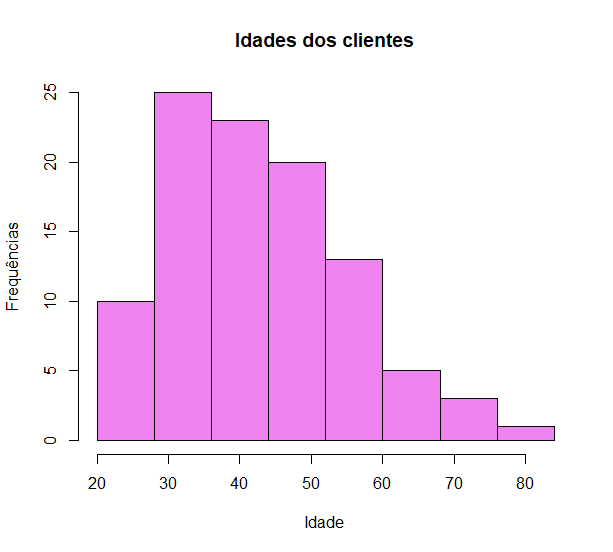
\includegraphics[keepaspectratio]{1.png}}
\caption{Alt text}
\end{figure}

==================================================================================================

\subsubsection{\texorpdfstring{Em seguida fiz uma analise descritiva das
frequências das varivéis qualitativas \texttt{Tipo\ de\ cliente},
\texttt{Método\ de\ pagamento}, \texttt{Gênero} e
\texttt{Estado\ civil}. Para nao repetir de criação de tabelas, criei
uma função que recebe o nome da variável e gera a tabela de
frequências.}{Em seguida fiz uma analise descritiva das frequências das varivéis qualitativas Tipo de cliente, Método de pagamento, Gênero e Estado civil. Para nao repetir de criação de tabelas, criei uma função que recebe o nome da variável e gera a tabela de frequências.}}\label{em-seguida-fiz-uma-analise-descritiva-das-frequuxeancias-das-varivuxe9is-qualitativas-tipo-de-cliente-muxe9todo-de-pagamento-guxeanero-e-estado-civil.-para-nao-repetir-de-criauxe7uxe3o-de-tabelas-criei-uma-funuxe7uxe3o-que-recebe-o-nome-da-variuxe1vel-e-gera-a-tabela-de-frequuxeancias.}

\begin{Shaded}
\begin{Highlighting}[]
\CommentTok{\#=============================================================}
\CommentTok{\# Análise de Frequências e Estatísticas Descritivas          |}
\CommentTok{\#=============================================================}
\NormalTok{criar\_tabela\_frequencia }\OtherTok{\textless{}{-}} \ControlFlowTok{function}\NormalTok{(dados, variavel) \{}
\NormalTok{  abs }\OtherTok{\textless{}{-}} \FunctionTok{table}\NormalTok{(dados[[variavel]])}
\NormalTok{  rel }\OtherTok{\textless{}{-}} \FunctionTok{prop.table}\NormalTok{(abs)}
\NormalTok{  rel\_perc }\OtherTok{\textless{}{-}}\NormalTok{ rel }\SpecialCharTok{*} \DecValTok{100}
  \FunctionTok{data.frame}\NormalTok{(}
    \AttributeTok{Categoria =} \FunctionTok{names}\NormalTok{(abs),}
    \AttributeTok{Frequencia\_Absoluta =} \FunctionTok{as.numeric}\NormalTok{(abs),}
    \AttributeTok{Frequencia\_Relativa =} \FunctionTok{round}\NormalTok{(}\FunctionTok{as.numeric}\NormalTok{(rel), }\DecValTok{4}\NormalTok{),}
    \AttributeTok{Frequencia\_Relativa\_Porcentagem =} \FunctionTok{round}\NormalTok{(}\FunctionTok{as.numeric}\NormalTok{(rel\_perc), }\DecValTok{2}\NormalTok{)}
\NormalTok{  )}
\NormalTok{\}}

\NormalTok{adicionar\_total }\OtherTok{\textless{}{-}} \ControlFlowTok{function}\NormalTok{(tabela) \{}
\NormalTok{  total }\OtherTok{\textless{}{-}} \FunctionTok{data.frame}\NormalTok{(}
    \AttributeTok{Categoria =} \StringTok{"Total"}\NormalTok{,}
    \AttributeTok{Frequencia\_Absoluta =} \FunctionTok{sum}\NormalTok{(tabela}\SpecialCharTok{$}\NormalTok{Frequencia\_Absoluta),}
    \AttributeTok{Frequencia\_Relativa =} \FunctionTok{sum}\NormalTok{(tabela}\SpecialCharTok{$}\NormalTok{Frequencia\_Relativa),}
    \AttributeTok{Frequencia\_Relativa\_Porcentagem =} \DecValTok{100}
\NormalTok{  )}
  \FunctionTok{rbind}\NormalTok{(tabela, total)}
\NormalTok{\}}

\CommentTok{\# Type of Customer}
\NormalTok{tabela\_customer }\OtherTok{\textless{}{-}} \FunctionTok{criar\_tabela\_frequencia}\NormalTok{(dados\_trabalho, }\StringTok{"Type.of.Customer"}\NormalTok{)}
\NormalTok{tabela\_customer }\OtherTok{\textless{}{-}} \FunctionTok{adicionar\_total}\NormalTok{(tabela\_customer)}

\CommentTok{\# Method of Payment}
\NormalTok{tabela\_payment }\OtherTok{\textless{}{-}} \FunctionTok{criar\_tabela\_frequencia}\NormalTok{(dados\_trabalho, }\StringTok{"Method.of.Payment"}\NormalTok{)}
\NormalTok{tabela\_payment }\OtherTok{\textless{}{-}} \FunctionTok{adicionar\_total}\NormalTok{(tabela\_payment)}

\CommentTok{\# Gender}
\NormalTok{tabela\_gender }\OtherTok{\textless{}{-}} \FunctionTok{criar\_tabela\_frequencia}\NormalTok{(dados\_trabalho, }\StringTok{"Gender"}\NormalTok{)}
\NormalTok{tabela\_gender }\OtherTok{\textless{}{-}} \FunctionTok{adicionar\_total}\NormalTok{(tabela\_gender)}

\CommentTok{\# Marital Status}
\NormalTok{tabela\_marital }\OtherTok{\textless{}{-}} \FunctionTok{criar\_tabela\_frequencia}\NormalTok{(dados\_trabalho, }\StringTok{"Marital.Status"}\NormalTok{)}
\NormalTok{tabela\_marital }\OtherTok{\textless{}{-}} \FunctionTok{adicionar\_total}\NormalTok{(tabela\_marital)}

\CommentTok{\#==================== tabela frequencia por cliente ====================\#}

\NormalTok{tabela\_cliente\_plot }\OtherTok{\textless{}{-}}\NormalTok{ tabela\_customer[tabela\_customer}\SpecialCharTok{$}\NormalTok{Categoria }\SpecialCharTok{!=} \StringTok{"Total"}\NormalTok{, ]}
\FunctionTok{barplot}\NormalTok{(}
\NormalTok{  tabela\_cliente\_plot}\SpecialCharTok{$}\NormalTok{Frequencia\_Absoluta,}
  \AttributeTok{names.arg =}\NormalTok{ tabela\_cliente\_plot}\SpecialCharTok{$}\NormalTok{Categoria,}
  \AttributeTok{main =} \StringTok{"Frequência por Tipo de Cliente"}\NormalTok{,}
  \AttributeTok{col =} \StringTok{"purple"}\NormalTok{,}
  \AttributeTok{las =} \DecValTok{2}\NormalTok{,}
  \AttributeTok{ylab =} \StringTok{"Frequência"}\NormalTok{,}
  \AttributeTok{xlab =} \StringTok{"Tipo de Cliente"}
\NormalTok{)}
\CommentTok{\#==================== tabela frequencia por metodo de pagamento ====================\#}

\FunctionTok{barplot}\NormalTok{(}
\NormalTok{  tabela\_payment}\SpecialCharTok{$}\NormalTok{Frequencia\_Absoluta[}\SpecialCharTok{{-}}\FunctionTok{nrow}\NormalTok{(tabela\_payment)],}
  \AttributeTok{names.arg =}\NormalTok{ tabela\_payment}\SpecialCharTok{$}\NormalTok{Categoria[}\SpecialCharTok{{-}}\FunctionTok{nrow}\NormalTok{(tabela\_payment)],}
  \AttributeTok{main =} \StringTok{"Método de Pagamento"}\NormalTok{,}
  \AttributeTok{col =} \StringTok{"red"}\NormalTok{,}
  \AttributeTok{las =} \DecValTok{2}\NormalTok{,}
  \AttributeTok{ylab =} \StringTok{"Frequência"}\NormalTok{,}
  \AttributeTok{xlab =} \StringTok{"Método"}
\NormalTok{)}
\CommentTok{\#==================== tabela frequencia por genero ====================\#}

\NormalTok{tabela\_gender\_plot }\OtherTok{\textless{}{-}}\NormalTok{ tabela\_gender[tabela\_gender}\SpecialCharTok{$}\NormalTok{Categoria }\SpecialCharTok{!=} \StringTok{"Total"}\NormalTok{, ]}
\FunctionTok{barplot}\NormalTok{(}
\NormalTok{    tabela\_gender\_plot}\SpecialCharTok{$}\NormalTok{Frequencia\_Absoluta,}
    \AttributeTok{names.arg =}\NormalTok{ tabela\_gender\_plot}\SpecialCharTok{$}\NormalTok{Categoria,}
    \AttributeTok{main =} \StringTok{"Frequência por Gênero"}\NormalTok{,}
    \AttributeTok{col =} \StringTok{"blue"}\NormalTok{,}
    \AttributeTok{las =} \DecValTok{2}\NormalTok{,}
    \AttributeTok{ylab =} \StringTok{"Frequência"}\NormalTok{,}
    \AttributeTok{xlab =} \StringTok{"Gênero"}
\NormalTok{)}

\CommentTok{\#==================== tabela frequencia por estado civil ====================\#}

\FunctionTok{barplot}\NormalTok{(}
\NormalTok{  tabela\_marital}\SpecialCharTok{$}\NormalTok{Frequencia\_Absoluta[}\SpecialCharTok{{-}}\FunctionTok{nrow}\NormalTok{(tabela\_marital)],}
  \AttributeTok{names.arg =}\NormalTok{ tabela\_marital}\SpecialCharTok{$}\NormalTok{Categoria[}\SpecialCharTok{{-}}\FunctionTok{nrow}\NormalTok{(tabela\_marital)],}
  \AttributeTok{main =} \StringTok{"Estado Civil"}\NormalTok{,}
  \AttributeTok{col =} \StringTok{"green"}\NormalTok{,}
  \AttributeTok{las =} \DecValTok{2}\NormalTok{,}
  \AttributeTok{ylab =} \StringTok{"Frequência"}\NormalTok{,}
  \AttributeTok{xlab =} \StringTok{"Estado Civil"}
\NormalTok{)}
\end{Highlighting}
\end{Shaded}

\pandocbounded{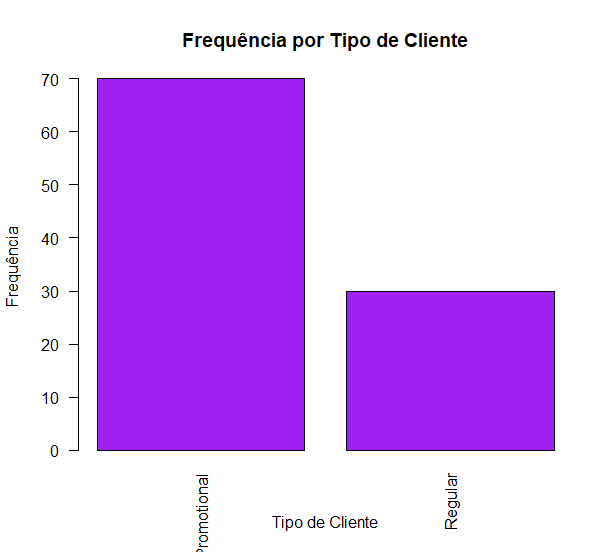
\includegraphics[keepaspectratio]{2.png}}
\pandocbounded{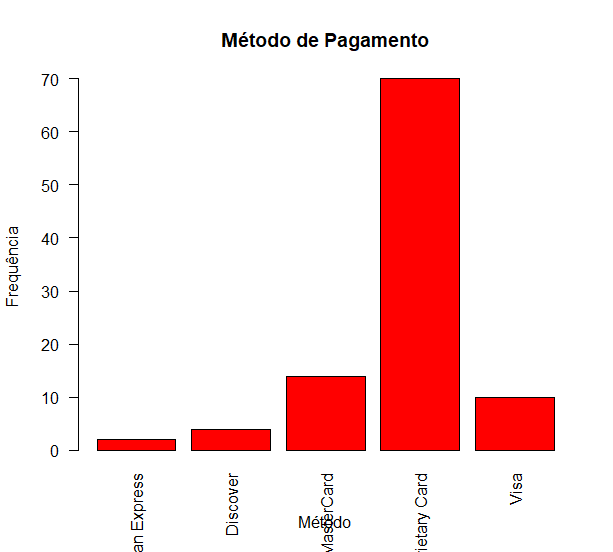
\includegraphics[keepaspectratio]{3.png}}
\pandocbounded{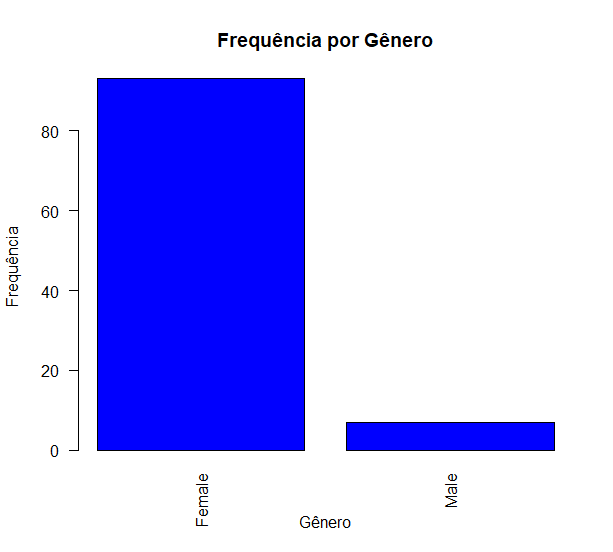
\includegraphics[keepaspectratio]{4.png}}
\pandocbounded{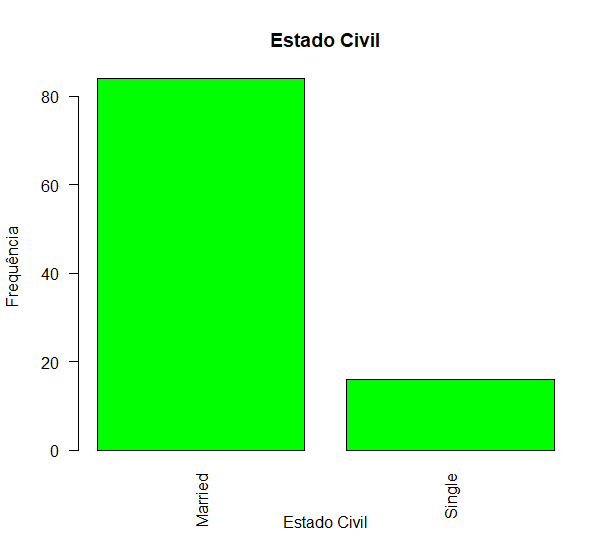
\includegraphics[keepaspectratio]{5.png}}

===================================================================================================

\subsubsection{Fiz uma relação entre Type of Customer e Net Sales. A
ideia é verificar se as vendas feitas para clientes promocionais
apresentam valores maiores do que a venda para clientes
regulares.}\label{fiz-uma-relauxe7uxe3o-entre-type-of-customer-e-net-sales.-a-ideia-uxe9-verificar-se-as-vendas-feitas-para-clientes-promocionais-apresentam-valores-maiores-do-que-a-venda-para-clientes-regulares.}

\begin{Shaded}
\begin{Highlighting}[]
\CommentTok{\#==================== Estatísticas Descritivas ====================}
\CommentTok{\# Type of customer x Net sales                                    |}
\CommentTok{\# Média, mediana e desvio padrão                                  |}
\CommentTok{\#==================================================================}
\NormalTok{dados\_trabalho}\SpecialCharTok{$}\NormalTok{Type.of.Customer }\OtherTok{\textless{}{-}} \FunctionTok{as.factor}\NormalTok{(dados\_trabalho}\SpecialCharTok{$}\NormalTok{Type.of.Customer)}
\NormalTok{dados\_trabalho}\SpecialCharTok{$}\NormalTok{Net.Sales }\OtherTok{\textless{}{-}} \FunctionTok{as.character}\NormalTok{(dados\_trabalho}\SpecialCharTok{$}\NormalTok{Net.Sales)}
\NormalTok{dados\_trabalho}\SpecialCharTok{$}\NormalTok{Net.Sales }\OtherTok{\textless{}{-}} \FunctionTok{gsub}\NormalTok{(}\StringTok{","}\NormalTok{, }\StringTok{"."}\NormalTok{, dados\_trabalho}\SpecialCharTok{$}\NormalTok{Net.Sales)}
\NormalTok{dados\_trabalho}\SpecialCharTok{$}\NormalTok{Net.Sales }\OtherTok{\textless{}{-}} \FunctionTok{as.numeric}\NormalTok{(dados\_trabalho}\SpecialCharTok{$}\NormalTok{Net.Sales)}

\FunctionTok{str}\NormalTok{(dados\_trabalho)}

\CommentTok{\# Estatísticas descritivas por grupo}
\NormalTok{media\_cada\_grupo }\OtherTok{\textless{}{-}} \FunctionTok{aggregate}\NormalTok{(Net.Sales }\SpecialCharTok{\textasciitilde{}}\NormalTok{ Type.of.Customer, }\AttributeTok{data =}\NormalTok{ dados\_trabalho, }\AttributeTok{FUN =}\NormalTok{ mean)}
\NormalTok{mediana\_por\_grupo }\OtherTok{\textless{}{-}} \FunctionTok{aggregate}\NormalTok{(Net.Sales }\SpecialCharTok{\textasciitilde{}}\NormalTok{ Type.of.Customer, }\AttributeTok{data =}\NormalTok{ dados\_trabalho, }\AttributeTok{FUN =}\NormalTok{ median)}
\NormalTok{desvio\_padrao\_por\_grupo }\OtherTok{\textless{}{-}} \FunctionTok{aggregate}\NormalTok{(Net.Sales }\SpecialCharTok{\textasciitilde{}}\NormalTok{ Type.of.Customer, }\AttributeTok{data =}\NormalTok{ dados\_trabalho, }\AttributeTok{FUN =}\NormalTok{ sd)}

\CommentTok{\# Teste t}
\NormalTok{teste }\OtherTok{\textless{}{-}} \FunctionTok{t.test}\NormalTok{(Net.Sales }\SpecialCharTok{\textasciitilde{}}\NormalTok{ Type.of.Customer, }\AttributeTok{data =}\NormalTok{ dados\_trabalho)}
\FunctionTok{cat}\NormalTok{(}\StringTok{"Teste entre grupos:}\SpecialCharTok{\textbackslash{}n}\StringTok{"}\NormalTok{)}
\FunctionTok{print}\NormalTok{(teste)}
\end{Highlighting}
\end{Shaded}

\subsubsection{Criei um boxplot para visualizar a distribuição das
vendas líquidas por tipo de
cliente.}\label{criei-um-boxplot-para-visualizar-a-distribuiuxe7uxe3o-das-vendas-luxedquidas-por-tipo-de-cliente.}

\begin{Shaded}
\begin{Highlighting}[]
\FunctionTok{source}\NormalTok{(}\StringTok{"analise.r"}\NormalTok{)}

\CommentTok{\#==================== boxplot vnedas x tipo cliente ====================\#}

\FunctionTok{boxplot}\NormalTok{(}
\NormalTok{  Net.Sales }\SpecialCharTok{\textasciitilde{}}\NormalTok{ Type.of.Customer,}
  \AttributeTok{data =}\NormalTok{ dados\_trabalho,}
  \AttributeTok{main =} \StringTok{"Net Sales por tipo de cliente"}\NormalTok{,}
  \AttributeTok{ylab =} \StringTok{"Vendas líquidas"}\NormalTok{,}
  \AttributeTok{xlab =} \StringTok{"Tipo de clientes"}\NormalTok{,}
  \AttributeTok{col =} \FunctionTok{c}\NormalTok{(}\StringTok{"\#ff7fff"}\NormalTok{, }\StringTok{"\#d64eff"}\NormalTok{)}
\NormalTok{)}
\end{Highlighting}
\end{Shaded}

\begin{figure}
\centering
\pandocbounded{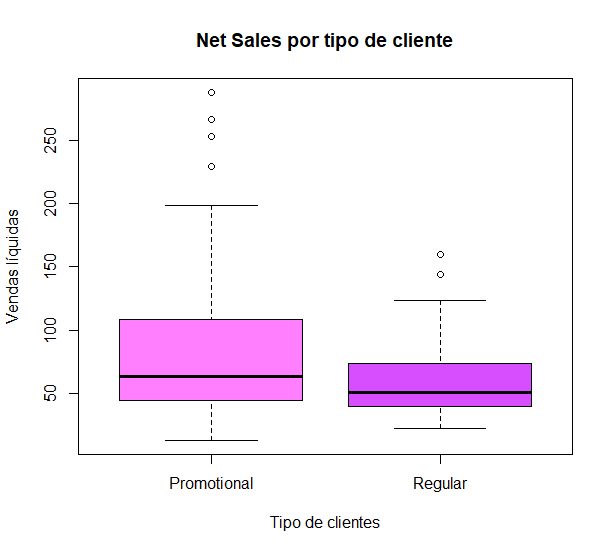
\includegraphics[keepaspectratio]{6.png}}
\caption{Alt text}
\end{figure}

\subsubsection{A saida para o teste t foi a
seguinte:}\label{a-saida-para-o-teste-t-foi-a-seguinte}

\begin{Shaded}
\begin{Highlighting}[]
\NormalTok{Teste entre grupos}\SpecialCharTok{:}

\NormalTok{        Welch Two Sample t}\SpecialCharTok{{-}}\NormalTok{test}

\NormalTok{data}\SpecialCharTok{:}\NormalTok{  Net.Sales by Type.of.Customer}
\NormalTok{t }\OtherTok{=} \FloatTok{2.2883}\NormalTok{, df }\OtherTok{=} \FloatTok{90.035}\NormalTok{, p}\SpecialCharTok{{-}}\NormalTok{value }\OtherTok{=} \FloatTok{0.02446}
\NormalTok{alternative hypothesis}\SpecialCharTok{:}\NormalTok{ true difference }\ControlFlowTok{in}\NormalTok{ means between group Promotional and group Regular is not equal to }\DecValTok{0}
\DecValTok{95}\NormalTok{ percent confidence interval}\SpecialCharTok{:}
  \FloatTok{2.939014} \FloatTok{41.657653}
\NormalTok{sample estimates}\SpecialCharTok{:}
\NormalTok{mean }\ControlFlowTok{in}\NormalTok{ group Promotional     mean }\ControlFlowTok{in}\NormalTok{ group Regular }
                 \FloatTok{84.29000}                  \FloatTok{61.99167}
\end{Highlighting}
\end{Shaded}

\begin{itemize}
\tightlist
\item
  Conclusão: Nesse caso de comparação tem uma diferença entre os grupos.
  Clientes Promotional gastaram mais em média que os Regular porque o
  p-valor baixo (\textless{} 0.05) e no intervalo de confiança que não
  inclui 0.
\end{itemize}

===================================================================================

\subsubsection{Nesse parte eu fiz uma distribuição de items na qual o
objetivo é entender como os clientes se comportam em relação à
quantidade de produtos adquiridos por
compra}\label{nesse-parte-eu-fiz-uma-distribuiuxe7uxe3o-de-items-na-qual-o-objetivo-uxe9-entender-como-os-clientes-se-comportam-em-relauxe7uxe3o-uxe0-quantidade-de-produtos-adquiridos-por-compra}

\begin{Shaded}
\begin{Highlighting}[]
\FunctionTok{source}\NormalTok{(}\StringTok{"analise.r"}\NormalTok{)}


\CommentTok{\#==================== distribuição de items ====================\#}
\FunctionTok{print}\NormalTok{(}\FunctionTok{ggplot}\NormalTok{(dados\_trabalho, }\FunctionTok{aes}\NormalTok{(}\AttributeTok{y =}\NormalTok{ Items)) }\SpecialCharTok{+}
  \FunctionTok{geom\_boxplot}\NormalTok{(}\AttributeTok{fill =} \StringTok{"lightblue"}\NormalTok{) }\SpecialCharTok{+}
  \FunctionTok{labs}\NormalTok{(}\AttributeTok{title =} \StringTok{"Distribuição de Items"}\NormalTok{, }\AttributeTok{y =} \StringTok{"Número de Items"}\NormalTok{))}

\FunctionTok{source}\NormalTok{(}\StringTok{"analise.r"}\NormalTok{)}

\CommentTok{\#==================== distribuição da freqência de items ====================\#}

\FunctionTok{print}\NormalTok{(}\FunctionTok{ggplot}\NormalTok{(dados\_trabalho, }\FunctionTok{aes}\NormalTok{(}\AttributeTok{x =}\NormalTok{ Items)) }\SpecialCharTok{+}
  \FunctionTok{geom\_histogram}\NormalTok{(}\FunctionTok{aes}\NormalTok{(}\AttributeTok{y =}\NormalTok{ ..density..), }\AttributeTok{binwidth =} \DecValTok{1}\NormalTok{, }\AttributeTok{fill =} \StringTok{"lightblue"}\NormalTok{, }\AttributeTok{color =} \StringTok{"black"}\NormalTok{) }\SpecialCharTok{+}
  \FunctionTok{geom\_density}\NormalTok{(}\AttributeTok{alpha =} \FloatTok{0.2}\NormalTok{, }\AttributeTok{fill =} \StringTok{"red"}\NormalTok{) }\SpecialCharTok{+}
  \FunctionTok{labs}\NormalTok{(}\AttributeTok{title =} \StringTok{"Distribuição de Itens por Compra"}\NormalTok{, }\AttributeTok{x =} \StringTok{"Número de Itens"}\NormalTok{, }\AttributeTok{y =} \StringTok{"Densidade"}\NormalTok{))}
\end{Highlighting}
\end{Shaded}

\pandocbounded{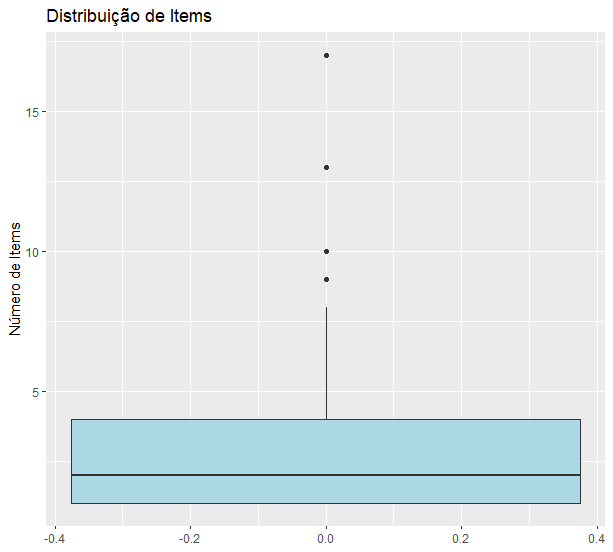
\includegraphics[keepaspectratio]{7.png}}
\pandocbounded{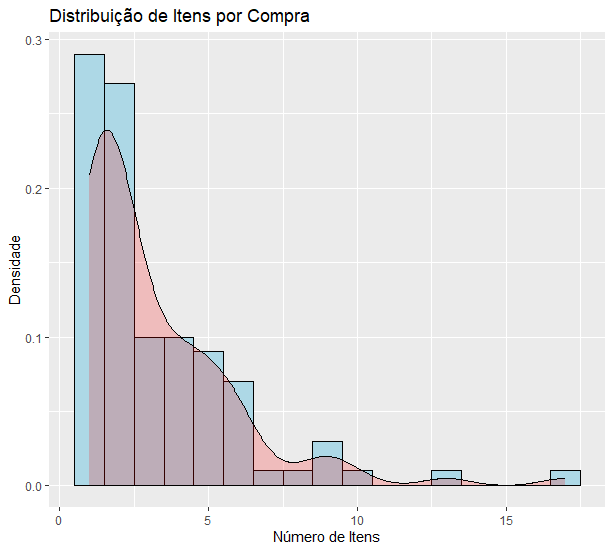
\includegraphics[keepaspectratio]{8.png}}

\subsubsection{Fiz também uma análise da quantidade de itens por
características qualitativas dos clientes. O objetivo é verificar se há
diferenças no comportamento de
compra}\label{fiz-tambuxe9m-uma-anuxe1lise-da-quantidade-de-itens-por-caracteruxedsticas-qualitativas-dos-clientes.-o-objetivo-uxe9-verificar-se-huxe1-diferenuxe7as-no-comportamento-de-compra}

\begin{Shaded}
\begin{Highlighting}[]

\CommentTok{\#==================== Itens x genêro ====================\#}

\FunctionTok{print}\NormalTok{(}
  \FunctionTok{ggplot}\NormalTok{(dados\_trabalho, }\FunctionTok{aes}\NormalTok{(}\AttributeTok{x =}\NormalTok{ Gender, }\AttributeTok{y =}\NormalTok{ Items, }\AttributeTok{fill =}\NormalTok{ Gender)) }\SpecialCharTok{+}
    \FunctionTok{geom\_boxplot}\NormalTok{() }\SpecialCharTok{+}
    \FunctionTok{labs}\NormalTok{(}\AttributeTok{title =} \StringTok{"Distribuição de Items por Gênero"}\NormalTok{, }\AttributeTok{x =} \StringTok{"Gênero"}\NormalTok{, }\AttributeTok{y =} \StringTok{"Número de Items"}\NormalTok{) }\SpecialCharTok{+}
    \FunctionTok{theme\_minimal}\NormalTok{()}
\NormalTok{)}

\CommentTok{\#==================== Itens x estado civil ====================\#}

\FunctionTok{print}\NormalTok{(}\FunctionTok{ggplot}\NormalTok{(dados\_trabalho, }\FunctionTok{aes}\NormalTok{(}\AttributeTok{x =}\NormalTok{ Marital.Status, }\AttributeTok{y =}\NormalTok{ Items, }\AttributeTok{fill =}\NormalTok{ Marital.Status)) }\SpecialCharTok{+}
  \FunctionTok{geom\_boxplot}\NormalTok{() }\SpecialCharTok{+}
  \FunctionTok{labs}\NormalTok{(}\AttributeTok{title =} \StringTok{"Distribuição de Items por Estado Civil"}\NormalTok{, }\AttributeTok{x =} \StringTok{"Estado Civil"}\NormalTok{, }\AttributeTok{y =} \StringTok{"Número de Items"}\NormalTok{) }\SpecialCharTok{+}
  \FunctionTok{theme\_minimal}\NormalTok{())}

\CommentTok{\#==================== Itens x tipo de cliente ====================\#}

\FunctionTok{print}\NormalTok{(}\FunctionTok{ggplot}\NormalTok{(dados\_trabalho, }\FunctionTok{aes}\NormalTok{(}\AttributeTok{x =}\NormalTok{ Type.of.Customer, }\AttributeTok{y =}\NormalTok{ Items, }\AttributeTok{fill =}\NormalTok{ Type.of.Customer)) }\SpecialCharTok{+}
  \FunctionTok{geom\_boxplot}\NormalTok{() }\SpecialCharTok{+}
  \FunctionTok{labs}\NormalTok{(}\AttributeTok{title =} \StringTok{"Distribuição de Items por Tipo de cliente"}\NormalTok{, }\AttributeTok{x =} \StringTok{"Tipo de cliente"}\NormalTok{, }\AttributeTok{y =} \StringTok{"Número de Items"}\NormalTok{) }\SpecialCharTok{+}
  \FunctionTok{theme\_minimal}\NormalTok{())}

\CommentTok{\#==================== Itens x método de pagamento ====================\#}

\FunctionTok{print}\NormalTok{(}\FunctionTok{ggplot}\NormalTok{(dados\_trabalho, }\FunctionTok{aes}\NormalTok{(}\AttributeTok{x =}\NormalTok{ Method.of.Payment, }\AttributeTok{y =}\NormalTok{ Items)) }\SpecialCharTok{+}
  \FunctionTok{geom\_boxplot}\NormalTok{() }\SpecialCharTok{+}
  \FunctionTok{labs}\NormalTok{(}\AttributeTok{title =} \StringTok{"Relação entre método de pagamento e número de itens"}\NormalTok{))}
\end{Highlighting}
\end{Shaded}

\pandocbounded{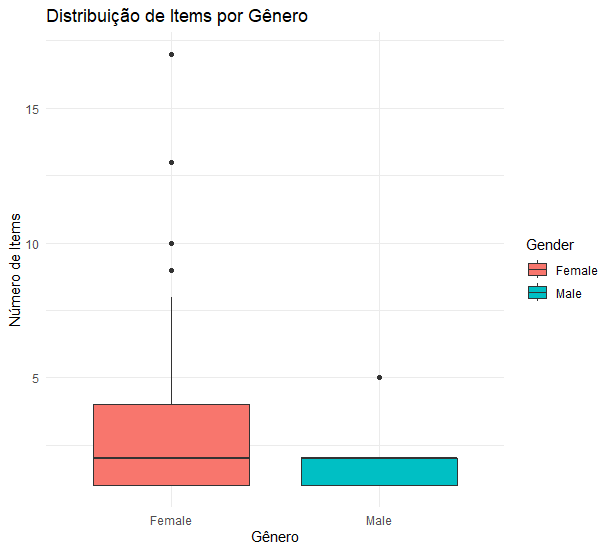
\includegraphics[keepaspectratio]{9.png}}
\pandocbounded{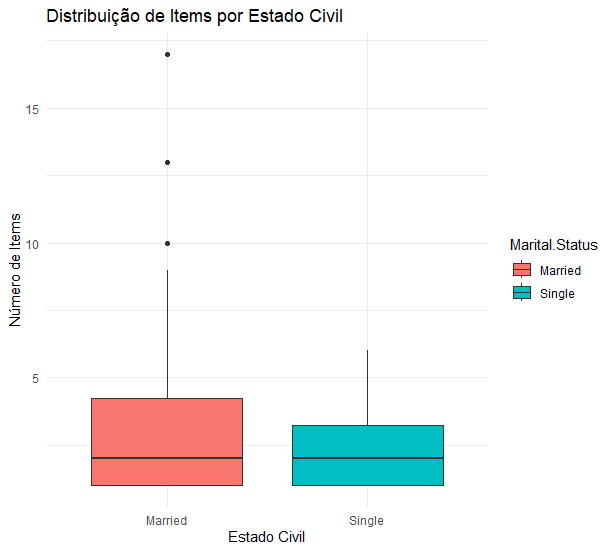
\includegraphics[keepaspectratio]{10.png}}
\pandocbounded{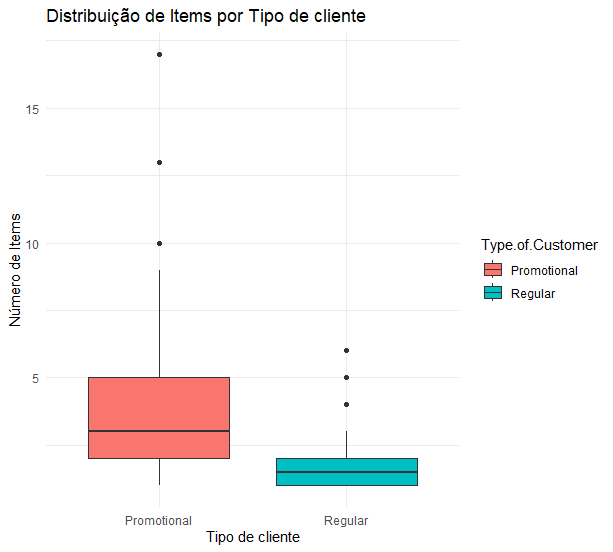
\includegraphics[keepaspectratio]{11.png}}
\pandocbounded{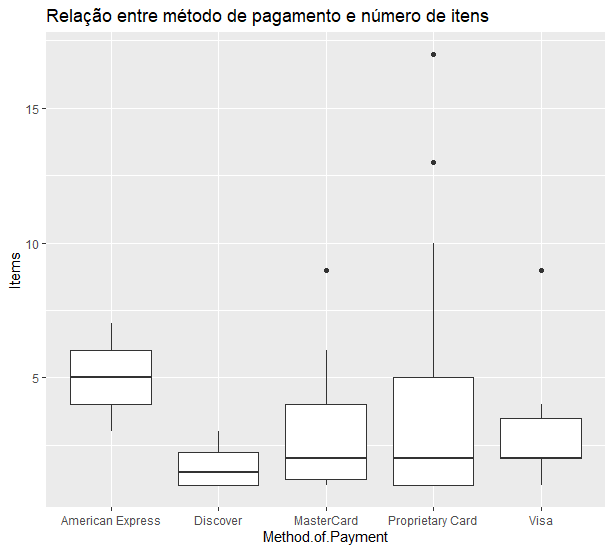
\includegraphics[keepaspectratio]{12.png}}

\subsection{Análisei da relação entre número de itens e vendas líquidas.
Nesta seção, eu analiso como o número de itens adquiridos em uma compra
se relaciona com as vendas líquidas. Utilizei uma correlação, um modelo
de regressão linear simples e visualização de um
grafico.}\label{anuxe1lisei-da-relauxe7uxe3o-entre-nuxfamero-de-itens-e-vendas-luxedquidas.-nesta-seuxe7uxe3o-eu-analiso-como-o-nuxfamero-de-itens-adquiridos-em-uma-compra-se-relaciona-com-as-vendas-luxedquidas.-utilizei-uma-correlauxe7uxe3o-um-modelo-de-regressuxe3o-linear-simples-e-visualizauxe7uxe3o-de-um-grafico.}

\subsubsection{Matriz de correlação - A matriz de correlação foi
calculada entre as variáveis Net.Sales, Items e Age, para avaliar a
força e a direção das relações lineares entre
elas.}\label{matriz-de-correlauxe7uxe3o---a-matriz-de-correlauxe7uxe3o-foi-calculada-entre-as-variuxe1veis-net.sales-items-e-age-para-avaliar-a-foruxe7a-e-a-direuxe7uxe3o-das-relauxe7uxf5es-lineares-entre-elas.}

\begin{Shaded}
\begin{Highlighting}[]
\NormalTok{correlacao }\OtherTok{\textless{}{-}} \FunctionTok{cor}\NormalTok{(dados\_trabalho[, }\FunctionTok{c}\NormalTok{(}\StringTok{"Net.Sales"}\NormalTok{, }\StringTok{"Items"}\NormalTok{, }\StringTok{"Age"}\NormalTok{)])}
\FunctionTok{diag}\NormalTok{(correlacao) }\OtherTok{\textless{}{-}} \ConstantTok{NA}
\FunctionTok{print}\NormalTok{(correlacao)}
\end{Highlighting}
\end{Shaded}

\subsubsection{Modelo linear simples - Foi ajustado um modelo de
regressão linear simples para prever as vendas líquidas a partir do
número de itens. O resumo do modelo mostra o quanto cada item adicional
impacta, em média, no valor das
vendas.}\label{modelo-linear-simples---foi-ajustado-um-modelo-de-regressuxe3o-linear-simples-para-prever-as-vendas-luxedquidas-a-partir-do-nuxfamero-de-itens.-o-resumo-do-modelo-mostra-o-quanto-cada-item-adicional-impacta-em-muxe9dia-no-valor-das-vendas.}

\begin{Shaded}
\begin{Highlighting}[]
\NormalTok{modelo\_final }\OtherTok{\textless{}{-}} \FunctionTok{lm}\NormalTok{(Net.Sales }\SpecialCharTok{\textasciitilde{}}\NormalTok{ Items, }\AttributeTok{data =}\NormalTok{ dados\_trabalho)}
\FunctionTok{summary}\NormalTok{(modelo\_final)}
\end{Highlighting}
\end{Shaded}

\subsubsection{Gráfico de dispersão com reta de regressão - O gráfico
abaixo mostra a relação entre o número de itens e as vendas líquidas,
com a reta ajustada pelo modelo
linear.}\label{gruxe1fico-de-dispersuxe3o-com-reta-de-regressuxe3o---o-gruxe1fico-abaixo-mostra-a-relauxe7uxe3o-entre-o-nuxfamero-de-itens-e-as-vendas-luxedquidas-com-a-reta-ajustada-pelo-modelo-linear.}

\begin{Shaded}
\begin{Highlighting}[]
\FunctionTok{library}\NormalTok{(ggplot2)}

\FunctionTok{ggplot}\NormalTok{(dados\_trabalho, }\FunctionTok{aes}\NormalTok{(}\AttributeTok{x =}\NormalTok{ Items, }\AttributeTok{y =}\NormalTok{ Net.Sales)) }\SpecialCharTok{+}
  \FunctionTok{geom\_point}\NormalTok{() }\SpecialCharTok{+}
  \FunctionTok{geom\_smooth}\NormalTok{(}\AttributeTok{method =} \StringTok{"lm"}\NormalTok{, }\AttributeTok{se =} \ConstantTok{FALSE}\NormalTok{, }\AttributeTok{color =} \StringTok{"red"}\NormalTok{) }\SpecialCharTok{+}
  \FunctionTok{labs}\NormalTok{(}\AttributeTok{title =} \StringTok{"Relação entre Número de Itens e Vendas Líquidas"}\NormalTok{,}
       \AttributeTok{x =} \StringTok{"Número de Itens"}\NormalTok{,}
       \AttributeTok{y =} \StringTok{"Vendas Líquidas (R$)"}\NormalTok{) }\SpecialCharTok{+}
  \FunctionTok{theme\_minimal}\NormalTok{()}
\end{Highlighting}
\end{Shaded}

\begin{Shaded}
\begin{Highlighting}[]
\CommentTok{\#==================== Gráfico: Itens x Vendas Líquidas ====================\#}
\FunctionTok{print}\NormalTok{(}\FunctionTok{ggplot}\NormalTok{(dados\_trabalho, }\FunctionTok{aes}\NormalTok{(}\AttributeTok{x =}\NormalTok{ Items, }\AttributeTok{y =}\NormalTok{ Net.Sales, }\AttributeTok{color =}\NormalTok{ Type.of.Customer)) }\SpecialCharTok{+}
  \FunctionTok{geom\_point}\NormalTok{() }\SpecialCharTok{+}
  \FunctionTok{geom\_smooth}\NormalTok{(}\AttributeTok{method =} \StringTok{"lm"}\NormalTok{, }\AttributeTok{se =} \ConstantTok{FALSE}\NormalTok{) }\SpecialCharTok{+}
  \FunctionTok{labs}\NormalTok{(}
    \AttributeTok{title =} \StringTok{"Relação entre Número de Itens e Valor Total da Compra"}\NormalTok{,}
    \AttributeTok{x =} \StringTok{"Quantidade de Itens"}\NormalTok{,}
    \AttributeTok{y =} \StringTok{"Vendas Líquidas (R$)"}\NormalTok{,}
    \AttributeTok{color =} \StringTok{"Tipo de Cliente"}
\NormalTok{  ) }\SpecialCharTok{+}
  \FunctionTok{scale\_color\_manual}\NormalTok{(}\AttributeTok{values =} \FunctionTok{c}\NormalTok{(}\StringTok{"Regular"} \OtherTok{=} \StringTok{"\#1f77b4"}\NormalTok{, }\StringTok{"Promotional"} \OtherTok{=} \StringTok{"\#ff7f0e"}\NormalTok{)) }\SpecialCharTok{+}
  \FunctionTok{theme\_minimal}\NormalTok{())}
\end{Highlighting}
\end{Shaded}

\pandocbounded{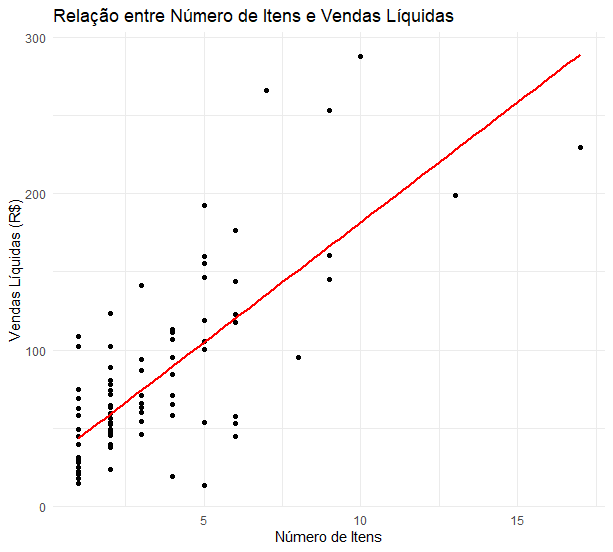
\includegraphics[keepaspectratio]{13.png}}
\pandocbounded{\includegraphics[keepaspectratio]{17.png}}

\subsubsection{Boxplot das vendas líquidas - Por fim, o boxplot abaixo
apresenta a distribuição das vendas líquidas, destacando a mediana, a
dispersão e possíveis
outliers.}\label{boxplot-das-vendas-luxedquidas---por-fim-o-boxplot-abaixo-apresenta-a-distribuiuxe7uxe3o-das-vendas-luxedquidas-destacando-a-mediana-a-dispersuxe3o-e-possuxedveis-outliers.}

\begin{Shaded}
\begin{Highlighting}[]
\FunctionTok{boxplot}\NormalTok{(dados\_trabalho}\SpecialCharTok{$}\NormalTok{Net.Sales, }
        \AttributeTok{main =} \StringTok{"Distribuição de Vendas Líquidas"}\NormalTok{, }
        \AttributeTok{col =} \StringTok{"pink"}\NormalTok{)}
\end{Highlighting}
\end{Shaded}

\begin{figure}
\centering
\pandocbounded{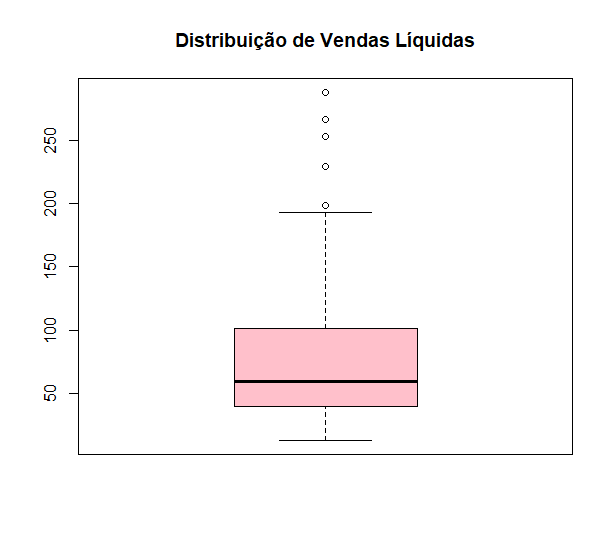
\includegraphics[keepaspectratio]{14.png}}
\caption{Alt text}
\end{figure}

\subsubsection{Aqui esta a saida esperada no
terminal}\label{aqui-esta-a-saida-esperada-no-terminal}

\begin{Shaded}
\begin{Highlighting}[]
\NormalTok{Matriz de correlação}\SpecialCharTok{:}
\NormalTok{            Net.Sales       Items         Age}
\NormalTok{Net.Sales          }\ConstantTok{NA}  \FloatTok{0.75505939} \SpecialCharTok{{-}}\FloatTok{0.01063589}
\NormalTok{Items      }\FloatTok{0.75505939}          \ConstantTok{NA} \SpecialCharTok{{-}}\FloatTok{0.01661542}
\NormalTok{Age       }\SpecialCharTok{{-}}\FloatTok{0.01063589} \SpecialCharTok{{-}}\FloatTok{0.01661542}          \ConstantTok{NA}
\NormalTok{Modelo final}\SpecialCharTok{:}

\NormalTok{Call}\SpecialCharTok{:}
\FunctionTok{lm}\NormalTok{(}\AttributeTok{formula =}\NormalTok{ Net.Sales }\SpecialCharTok{\textasciitilde{}}\NormalTok{ Items, }\AttributeTok{data =}\NormalTok{ dados\_trabalho)}

\NormalTok{Residuals}\SpecialCharTok{:}
\NormalTok{    Min      }\DecValTok{1}\NormalTok{Q  Median      }\DecValTok{3}\NormalTok{Q     Max}
\SpecialCharTok{{-}}\FloatTok{91.713} \SpecialCharTok{{-}}\FloatTok{19.450}  \SpecialCharTok{{-}}\FloatTok{4.851}  \FloatTok{15.710} \FloatTok{130.334}

\NormalTok{Coefficients}\SpecialCharTok{:}
\NormalTok{            Estimate Std. Error t value }\FunctionTok{Pr}\NormalTok{(}\SpecialCharTok{\textgreater{}}\ErrorTok{|}\NormalTok{t}\SpecialCharTok{|}\NormalTok{)    }
\NormalTok{(Intercept)   }\FloatTok{28.138}      \FloatTok{5.682}   \FloatTok{4.952} \FloatTok{3.06e{-}06} \SpecialCharTok{**}\ErrorTok{*}
\NormalTok{Items         }\FloatTok{15.361}      \FloatTok{1.347}  \FloatTok{11.400}  \SpecialCharTok{\textless{}} \FloatTok{2e{-}16} \SpecialCharTok{**}\ErrorTok{*}
\SpecialCharTok{{-}{-}{-}}
\NormalTok{Signif. codes}\SpecialCharTok{:}  \DecValTok{0} \StringTok{\textquotesingle{}***\textquotesingle{}} \FloatTok{0.001} \StringTok{\textquotesingle{}**\textquotesingle{}} \FloatTok{0.01} \StringTok{\textquotesingle{}*\textquotesingle{}} \FloatTok{0.05} \StringTok{\textquotesingle{}.\textquotesingle{}} \FloatTok{0.1} \StringTok{\textquotesingle{} \textquotesingle{}} \DecValTok{1}

\NormalTok{Residual standard error}\SpecialCharTok{:} \FloatTok{36.68}\NormalTok{ on }\DecValTok{98}\NormalTok{ degrees of freedom}
\NormalTok{Multiple R}\SpecialCharTok{{-}}\NormalTok{squared}\SpecialCharTok{:}  \FloatTok{0.5701}\NormalTok{,    Adjusted R}\SpecialCharTok{{-}}\NormalTok{squared}\SpecialCharTok{:}  \FloatTok{0.5657} 
\NormalTok{F}\SpecialCharTok{{-}}\NormalTok{statistic}\SpecialCharTok{:}   \DecValTok{130}\NormalTok{ on }\DecValTok{1}\NormalTok{ and }\DecValTok{98}\NormalTok{ DF,  p}\SpecialCharTok{{-}}\NormalTok{value}\SpecialCharTok{:} \ErrorTok{\textless{}} \FloatTok{2.2e{-}16}
\end{Highlighting}
\end{Shaded}

\subsubsection{Matriz de Correlação}\label{matriz-de-correlauxe7uxe3o}

Vemos na matriz de correlação entre as variáveis \emph{Net.Sales},
\emph{Items} e \emph{Age} que a maior correlação é entre
\emph{Net.Sales} e \emph{Items} (0,755), o que indica que as vendas
líquidas aumentam à medida que mais itens são vendidos. As correlações
com \emph{Age} são todas próximas de zero, o que nos diz que a idade dos
clientes não tem relação linear com as vendas nem com a quantidade de
itens.

\subsubsection{Regressão Linear de Vendas por
Itens}\label{regressuxe3o-linear-de-vendas-por-itens}

Um modelo de regressão linear simples foi ajustado para prever as vendas
(\emph{Net.Sales}) a partir do número de itens vendidos (\emph{Items}).
O modelo ajustado foi:

\[
\text{Net.Sales} = 28.14 + 15.36 \cdot \text{Items}
\]

Ou seja, para cada item adicional vendido, a venda aumenta em média R\$
15,36. O modelo explica cerca de 57\% da variação nas vendas (\emph{R² =
0.57}) e é estatisticamente significativo (p \textless{} 0.001), o que
significa que a quantidade de itens vendidos é um bom preditor do valor
das vendas.

====================================================================

\subsubsection{Como foi pedido no trabalho e lendo alguns artigos,
decidi implementar uma variavel aleatorio de início Loyalty Score porém
ela não se relacionou com uma precisão de venda boa, então decidi trocar
por varivel Ticket Médio, que é uma métrica importante para entender o
comportamento de compra dos clientes. O Ticket Médio é calculado
dividindo o total de vendas pelo número de transações realizadas. Essa
métrica ajuda a identificar o valor médio gasto por cliente em cada
compra. Essa variável foi muito útil para a analise, já que na minha
perspectiva seria de aumentar o lucro da
empresa.}\label{como-foi-pedido-no-trabalho-e-lendo-alguns-artigos-decidi-implementar-uma-variavel-aleatorio-de-inuxedcio-loyalty-score-poruxe9m-ela-nuxe3o-se-relacionou-com-uma-precisuxe3o-de-venda-boa-entuxe3o-decidi-trocar-por-varivel-ticket-muxe9dio-que-uxe9-uma-muxe9trica-importante-para-entender-o-comportamento-de-compra-dos-clientes.-o-ticket-muxe9dio-uxe9-calculado-dividindo-o-total-de-vendas-pelo-nuxfamero-de-transauxe7uxf5es-realizadas.-essa-muxe9trica-ajuda-a-identificar-o-valor-muxe9dio-gasto-por-cliente-em-cada-compra.-essa-variuxe1vel-foi-muito-uxfatil-para-a-analise-juxe1-que-na-minha-perspectiva-seria-de-aumentar-o-lucro-da-empresa.}

\subsubsection{Criação das novas
variáveis}\label{criauxe7uxe3o-das-novas-variuxe1veis}

\begin{itemize}
\item
  Age\_Group: você criou uma variável categórica com faixas etárias
  (idade\_classes), para facilitar análises por idade.
\item
  Ticket\_Medio: calcula o valor médio pago por item em cada compra,
  dividindo Net.Sales pelo número de Items. Essa métrica ajuda a
  entender o ``tamanho'' médio do gasto por item.
\item
  Cliente\_premium: marca os clientes no quartil superior das vendas
  líquidas como Premium (acima do 75º percentil) e os demais como
  Regular. Essa segmentação permite analisar diferenças entre clientes
  de maior e menor valor.
\end{itemize}

\begin{Shaded}
\begin{Highlighting}[]
\NormalTok{dados\_trabalho }\OtherTok{\textless{}{-}}\NormalTok{ dados\_trabalho }\SpecialCharTok{\%\textgreater{}\%} 
  \FunctionTok{mutate}\NormalTok{(}
    \AttributeTok{Age\_Group =}\NormalTok{ idade\_classes,  }
    \AttributeTok{Ticket\_Medio =}\NormalTok{ Net.Sales }\SpecialCharTok{/}\NormalTok{ Items,}
    \AttributeTok{Cliente\_premium =} \FunctionTok{ifelse}\NormalTok{(Net.Sales }\SpecialCharTok{\textgreater{}} \FunctionTok{quantile}\NormalTok{(Net.Sales, }\FloatTok{0.75}\NormalTok{), }\StringTok{"Premium"}\NormalTok{, }\StringTok{"Regular"}\NormalTok{)}
\NormalTok{  )}
\end{Highlighting}
\end{Shaded}

\subsection{Boxplot: Ticket Médio por Tipo de
Cliente}\label{boxplot-ticket-muxe9dio-por-tipo-de-cliente}

\subsubsection{Esse gráfico compara o Ticket Médio entre os dois tipos
de cliente (Promotional e Regular),
visualizando:}\label{esse-gruxe1fico-compara-o-ticket-muxe9dio-entre-os-dois-tipos-de-cliente-promotional-e-regular-visualizando}

\begin{itemize}
\item
  Diferenças de mediana.
\item
  Dispersão.
\item
  Outliers (dados que se diferenciam drasticamente de todos os outros).
\end{itemize}

Serve para identificar se clientes regulares ou promocionais tendem a
gastar mais por item.

\begin{Shaded}
\begin{Highlighting}[]
\FunctionTok{ggplot}\NormalTok{(dados\_trabalho, }\FunctionTok{aes}\NormalTok{(}\AttributeTok{x =}\NormalTok{ Type.of.Customer, }\AttributeTok{y =}\NormalTok{ Ticket\_Medio, }\AttributeTok{fill =}\NormalTok{ Type.of.Customer)) }\SpecialCharTok{+} 
  \FunctionTok{geom\_boxplot}\NormalTok{() }\SpecialCharTok{+}
  \FunctionTok{labs}\NormalTok{(}
    \AttributeTok{title =} \StringTok{"Nova análise: Ticket por Tipo de Cliente"}\NormalTok{,}
    \AttributeTok{y =} \StringTok{"R$ por item"}
\NormalTok{  ) }\SpecialCharTok{+}
  \FunctionTok{theme\_minimal}\NormalTok{()}
\end{Highlighting}
\end{Shaded}

\begin{figure}
\centering
\pandocbounded{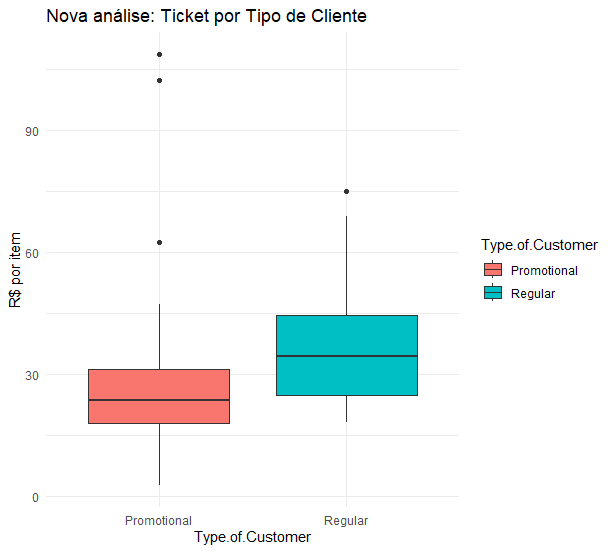
\includegraphics[keepaspectratio]{15.png}}
\caption{Alt text}
\end{figure}

\subsubsection{Teste estatístico: diferença no Ticket
Médio}\label{teste-estatuxedstico-diferenuxe7a-no-ticket-muxe9dio}

\begin{Shaded}
\begin{Highlighting}[]
\NormalTok{t\_test\_result }\OtherTok{\textless{}{-}} \FunctionTok{t.test}\NormalTok{(Ticket\_Medio }\SpecialCharTok{\textasciitilde{}}\NormalTok{ Type.of.Customer, }\AttributeTok{data =}\NormalTok{ dados\_trabalho)}
\end{Highlighting}
\end{Shaded}

\begin{itemize}
\item
  Testa se a média do Ticket Médio difere significativamente entre
  clientes Promotional e Regular.
\item
  Se o p-valor \textless{} 0,05, você conclui que existe diferença
  estatisticamente significativa.
\end{itemize}

\subsubsection{Regressão: Ticket Médio por Tipo de
Cliente}\label{regressuxe3o-ticket-muxe9dio-por-tipo-de-cliente}

\begin{Shaded}
\begin{Highlighting}[]
\NormalTok{modelo\_estrategico\_ticket\_medio }\OtherTok{\textless{}{-}} \FunctionTok{lm}\NormalTok{(Ticket\_Medio }\SpecialCharTok{\textasciitilde{}}\NormalTok{ Type.of.Customer, }\AttributeTok{data =}\NormalTok{ dados\_trabalho)}
\end{Highlighting}
\end{Shaded}

\begin{itemize}
\item
  Modelo simples para quantificar o impacto de ser Promotional ou
  Regular sobre o Ticket Médio.
\item
  Complementa o t-test, mas com uma análise mais formal e possibilitando
  ver os coeficientes.
\end{itemize}

\subsubsection{Gráfico: Método de Pagamento por Status
Premium}\label{gruxe1fico-muxe9todo-de-pagamento-por-status-premium}

\begin{Shaded}
\begin{Highlighting}[]
  \FunctionTok{ggplot}\NormalTok{(dados\_trabalho, }\FunctionTok{aes}\NormalTok{(}\AttributeTok{x =}\NormalTok{ Method.of.Payment, }\AttributeTok{fill =}\NormalTok{ Cliente\_premium)) }\SpecialCharTok{+}
    \FunctionTok{geom\_bar}\NormalTok{(}\AttributeTok{position =} \StringTok{"fill"}\NormalTok{) }\SpecialCharTok{+}
    \FunctionTok{labs}\NormalTok{(}
      \AttributeTok{title =} \StringTok{"Nova análise: Métodos de Pagamento por Status Premium"}\NormalTok{,}
      \AttributeTok{y =} \StringTok{"Proporção"}
\NormalTok{    ) }\SpecialCharTok{+}
    \FunctionTok{theme\_minimal}\NormalTok{() }\SpecialCharTok{+}
    \FunctionTok{theme}\NormalTok{(}\AttributeTok{axis.text.x =} \FunctionTok{element\_text}\NormalTok{(}\AttributeTok{angle =} \DecValTok{45}\NormalTok{, }\AttributeTok{hjust =} \DecValTok{1}\NormalTok{))}
\end{Highlighting}
\end{Shaded}

\begin{figure}
\centering
\pandocbounded{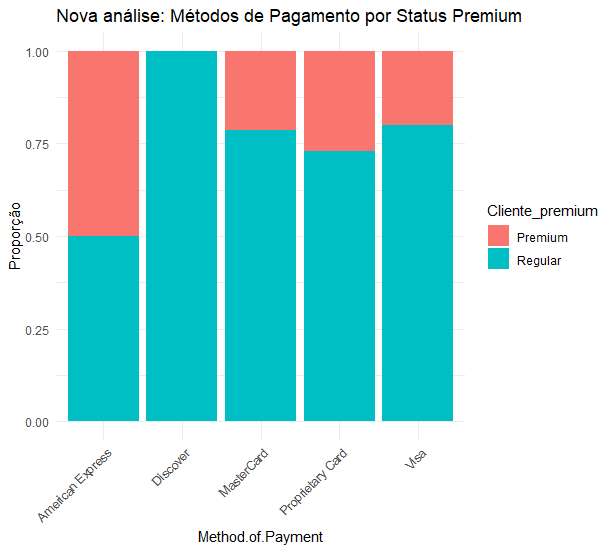
\includegraphics[keepaspectratio]{16.png}}
\caption{Alt text}
\end{figure}

\begin{itemize}
\item
  Mostra a proporção dos métodos de pagamento usados, separados entre
  clientes Premium e Regular.
\item
  Ajuda a entender se clientes Premium têm preferência por algum método
  (ex.: cartão proprietário)
\end{itemize}

\subsubsection{Modelo de regressão
múltipla}\label{modelo-de-regressuxe3o-muxfaltipla}

\begin{Shaded}
\begin{Highlighting}[]
\NormalTok{modelo\_estrategico }\OtherTok{\textless{}{-}} \FunctionTok{lm}\NormalTok{(Net.Sales }\SpecialCharTok{\textasciitilde{}}\NormalTok{ Items }\SpecialCharTok{+}\NormalTok{ Ticket\_Medio }\SpecialCharTok{+}\NormalTok{ Cliente\_premium, }\AttributeTok{data =}\NormalTok{ dados\_trabalho)}
\end{Highlighting}
\end{Shaded}

Modelo mais completo para prever as Net.Sales, considerando:

\begin{itemize}
\item
  Número de itens.
\item
  Ticket médio.
\item
  Status Premium.
\end{itemize}

Permite identificar quais dessas variáveis têm maior impacto nas vendas
e se elas explicam bem a variação observada.

\begin{Shaded}
\begin{Highlighting}[]
\NormalTok{[}\DecValTok{1}\NormalTok{] }\StringTok{"TESTE NOVO: Diferença no Ticket entre Clientes Regulares e Promocionais"}

\NormalTok{        Welch Two Sample t}\SpecialCharTok{{-}}\NormalTok{test}

\NormalTok{data}\SpecialCharTok{:}\NormalTok{  Ticket\_Medio by Type.of.Customer}
\NormalTok{t }\OtherTok{=} \SpecialCharTok{{-}}\FloatTok{2.9749}\NormalTok{, df }\OtherTok{=} \FloatTok{61.267}\NormalTok{, p}\SpecialCharTok{{-}}\NormalTok{value }\OtherTok{=} \FloatTok{0.004189}
\NormalTok{alternative hypothesis}\SpecialCharTok{:}\NormalTok{ true difference }\ControlFlowTok{in}\NormalTok{ means between group Promotional and group Regular is not equal to }\DecValTok{0}
\DecValTok{95}\NormalTok{ percent confidence interval}\SpecialCharTok{:}
 \SpecialCharTok{{-}}\FloatTok{17.114367}  \SpecialCharTok{{-}}\FloatTok{3.356147}
\NormalTok{sample estimates}\SpecialCharTok{:}
\NormalTok{mean }\ControlFlowTok{in}\NormalTok{ group Promotional     mean }\ControlFlowTok{in}\NormalTok{ group Regular }
                 \FloatTok{26.55197}                  \FloatTok{36.78722}

\NormalTok{[}\DecValTok{1}\NormalTok{] }\StringTok{"Modelo Estratégico: Ticket Médio por Tipo de Cliente}\SpecialCharTok{\textbackslash{}n}\StringTok{"}

\NormalTok{Call}\SpecialCharTok{:}
\FunctionTok{lm}\NormalTok{(}\AttributeTok{formula =}\NormalTok{ Ticket\_Medio }\SpecialCharTok{\textasciitilde{}}\NormalTok{ Type.of.Customer, }\AttributeTok{data =}\NormalTok{ dados\_trabalho)}

\NormalTok{Residuals}\SpecialCharTok{:}
\NormalTok{    Min      }\DecValTok{1}\NormalTok{Q  Median      }\DecValTok{3}\NormalTok{Q     Max}
\SpecialCharTok{{-}}\FloatTok{23.906} \SpecialCharTok{{-}}\FloatTok{10.294}  \SpecialCharTok{{-}}\FloatTok{2.885}   \FloatTok{5.048}  \FloatTok{82.248}

\NormalTok{Coefficients}\SpecialCharTok{:}
\NormalTok{                        Estimate Std. Error t value }\FunctionTok{Pr}\NormalTok{(}\SpecialCharTok{\textgreater{}}\ErrorTok{|}\NormalTok{t}\SpecialCharTok{|}\NormalTok{)    }
\NormalTok{(Intercept)               }\FloatTok{26.552}      \FloatTok{1.974}   \FloatTok{13.45}  \SpecialCharTok{\textless{}} \FloatTok{2e{-}16} \SpecialCharTok{**}\ErrorTok{*}
\NormalTok{Type.of.CustomerRegular   }\FloatTok{10.235}      \FloatTok{3.604}    \FloatTok{2.84}  \FloatTok{0.00549} \SpecialCharTok{**}
\SpecialCharTok{{-}{-}{-}}
\NormalTok{Signif. codes}\SpecialCharTok{:}  \DecValTok{0} \StringTok{\textquotesingle{}***\textquotesingle{}} \FloatTok{0.001} \StringTok{\textquotesingle{}**\textquotesingle{}} \FloatTok{0.01} \StringTok{\textquotesingle{}*\textquotesingle{}} \FloatTok{0.05} \StringTok{\textquotesingle{}.\textquotesingle{}} \FloatTok{0.1} \StringTok{\textquotesingle{} \textquotesingle{}} \DecValTok{1}

\NormalTok{Residual standard error}\SpecialCharTok{:} \FloatTok{16.52}\NormalTok{ on }\DecValTok{98}\NormalTok{ degrees of freedom}
\NormalTok{Multiple R}\SpecialCharTok{{-}}\NormalTok{squared}\SpecialCharTok{:}  \FloatTok{0.07603}\NormalTok{,   Adjusted R}\SpecialCharTok{{-}}\NormalTok{squared}\SpecialCharTok{:}  \FloatTok{0.0666} 
\NormalTok{F}\SpecialCharTok{{-}}\NormalTok{statistic}\SpecialCharTok{:} \FloatTok{8.064}\NormalTok{ on }\DecValTok{1}\NormalTok{ and }\DecValTok{98}\NormalTok{ DF,  p}\SpecialCharTok{{-}}\NormalTok{value}\SpecialCharTok{:} \FloatTok{0.00549}

\NormalTok{[}\DecValTok{1}\NormalTok{] }\StringTok{"MODELO NOVO: Impacto do Ticket e Status Premium nas Vendas"}

\NormalTok{Call}\SpecialCharTok{:}
\FunctionTok{lm}\NormalTok{(}\AttributeTok{formula =}\NormalTok{ Net.Sales }\SpecialCharTok{\textasciitilde{}}\NormalTok{ Items }\SpecialCharTok{+}\NormalTok{ Ticket\_Medio }\SpecialCharTok{+}\NormalTok{ Cliente\_premium,}
    \AttributeTok{data =}\NormalTok{ dados\_trabalho)}

\NormalTok{Residuals}\SpecialCharTok{:}
\NormalTok{    Min      }\DecValTok{1}\NormalTok{Q  Median      }\DecValTok{3}\NormalTok{Q     Max }
\SpecialCharTok{{-}}\FloatTok{51.746}  \SpecialCharTok{{-}}\FloatTok{7.065}  \SpecialCharTok{{-}}\FloatTok{3.679}   \FloatTok{9.479}  \FloatTok{94.165}

\NormalTok{Coefficients}\SpecialCharTok{:}
\NormalTok{                       Estimate Std. Error t value }\FunctionTok{Pr}\NormalTok{(}\SpecialCharTok{\textgreater{}}\ErrorTok{|}\NormalTok{t}\SpecialCharTok{|}\NormalTok{)}
\NormalTok{(Intercept)             }\FloatTok{44.3524}    \FloatTok{13.5910}   \FloatTok{3.263}  \FloatTok{0.00153} \SpecialCharTok{**} 
\NormalTok{Items                   }\FloatTok{13.0849}     \FloatTok{1.3325}   \FloatTok{9.820} \FloatTok{3.63e{-}16} \SpecialCharTok{**}\ErrorTok{*}
\NormalTok{Ticket\_Medio             }\FloatTok{0.9444}     \FloatTok{0.1768}   \FloatTok{5.341} \FloatTok{6.19e{-}07} \SpecialCharTok{**}\ErrorTok{*}
\NormalTok{Cliente\_premiumRegular }\SpecialCharTok{{-}}\FloatTok{49.1486}     \FloatTok{7.8802}  \SpecialCharTok{{-}}\FloatTok{6.237} \FloatTok{1.20e{-}08} \SpecialCharTok{**}\ErrorTok{*}
\SpecialCharTok{{-}{-}{-}}
\NormalTok{Signif. codes}\SpecialCharTok{:}  \DecValTok{0} \StringTok{\textquotesingle{}***\textquotesingle{}} \FloatTok{0.001} \StringTok{\textquotesingle{}**\textquotesingle{}} \FloatTok{0.01} \StringTok{\textquotesingle{}*\textquotesingle{}} \FloatTok{0.05} \StringTok{\textquotesingle{}.\textquotesingle{}} \FloatTok{0.1} \StringTok{\textquotesingle{} \textquotesingle{}} \DecValTok{1}

\NormalTok{Residual standard error}\SpecialCharTok{:} \FloatTok{23.18}\NormalTok{ on }\DecValTok{96}\NormalTok{ degrees of freedom}
\NormalTok{Multiple R}\SpecialCharTok{{-}}\NormalTok{squared}\SpecialCharTok{:}  \FloatTok{0.8319}\NormalTok{,    Adjusted R}\SpecialCharTok{{-}}\NormalTok{squared}\SpecialCharTok{:}  \FloatTok{0.8267}
\NormalTok{F}\SpecialCharTok{{-}}\NormalTok{statistic}\SpecialCharTok{:} \FloatTok{158.4}\NormalTok{ on }\DecValTok{3}\NormalTok{ and }\DecValTok{96}\NormalTok{ DF,  p}\SpecialCharTok{{-}}\NormalTok{value}\SpecialCharTok{:} \ErrorTok{\textless{}} \FloatTok{2.2e{-}16}
\end{Highlighting}
\end{Shaded}

\subsection{Resultado das Análises
Adicionais}\label{resultado-das-anuxe1lises-adicionais}

\subsubsection{1. Teste t para o Ticket Médio por Tipo de
Cliente}\label{teste-t-para-o-ticket-muxe9dio-por-tipo-de-cliente}

Realizamos um \textbf{teste t de Welch} para verificar se o ticket médio
(\emph{venda média por item}) difere entre clientes
\textbf{promocionais} e \textbf{regulares}.

Os resultados mostram:

\begin{itemize}
\tightlist
\item
  Média dos clientes \textbf{Promocionais}: 26,55
\item
  Média dos clientes \textbf{Regulares}: 36,79
\item
  Estatística t = -2,97\\
\item
  p-valor = 0,004
\end{itemize}

Como o p-valor é menor que 0,05, concluímos que existe uma diferença
estatisticamente significativa no ticket médio entre os dois grupos,
indicando que clientes regulares tendem a gastar mais por item do que
clientes promocionais.

\begin{center}\rule{0.5\linewidth}{0.5pt}\end{center}

\subsubsection{2. Regressão Linear Simples: Ticket Médio por Tipo de
Cliente}\label{regressuxe3o-linear-simples-ticket-muxe9dio-por-tipo-de-cliente}

Ajustamos um modelo de regressão para quantificar a diferença no ticket
médio entre os grupos. O modelo é dado por:

\[
\text{Ticket Médio} = \beta_0 + \beta_1 (\text{Cliente Regular})
\]

\begin{itemize}
\tightlist
\item
  Intercepto (\(\beta_0\)): 26,55 → ticket médio dos
  \textbf{promocionais}
\item
  Coeficiente para \textbf{Cliente Regular}: +10,24, com p-valor ≈ 0,005
\end{itemize}

Ou seja, ser um cliente regular está associado a um aumento médio de
aproximadamente 10,24 unidades monetárias no ticket médio em relação aos
promocionais. Esse resultado confirma o teste t.

O modelo explica cerca de 7,6\% da variação no ticket médio
\((R^2 ≈ 0,076)\).

\begin{center}\rule{0.5\linewidth}{0.5pt}\end{center}

\subsubsection{3. Regressão Múltipla: Impacto do Ticket e Status Premium
nas Vendas
Líquidas}\label{regressuxe3o-muxfaltipla-impacto-do-ticket-e-status-premium-nas-vendas-luxedquidas}

Por fim, ajustamos um modelo mais completo para explicar as
\textbf{vendas líquidas}, incluindo como variáveis explicativas: número
de itens comprados, ticket médio e status premium do cliente.

O modelo é dado por:

\[
\text{Net Sales} = \beta_0 + \beta_1 (\text{Items}) + \beta_2 (\text{Ticket Médio}) + \beta_3 (\text{Cliente Premium})
\]

Os principais resultados:

\begin{itemize}
\tightlist
\item
  Para cada item adicional, as vendas líquidas aumentam, em média,
  13,08.
\item
  Para cada unidade monetária a mais no ticket médio, as vendas líquidas
  aumentam, em média, 0,94.
\item
  Clientes regulares (em relação aos premium) têm em média 49,15 a menos
  em vendas líquidas.
\item
  O modelo tem \((R^2 ≈ 0,83)\), explicando mais de 80\% da variação nas
  vendas líquidas, o que indica um bom ajuste.
\end{itemize}

\begin{center}\rule{0.5\linewidth}{0.5pt}\end{center}

\subsection{Resumo}\label{resumo}

As análises revelam que:

\begin{itemize}
\tightlist
\item
  Clientes regulares tendem a ter um ticket médio maior do que os
  promocionais.
\item
  O número de itens, o ticket médio e o status premium são fatores
  importantes para explicar as vendas líquidas.
\item
  O modelo múltiplo mostra que essas variáveis, em conjunto, têm grande
  poder explicativo das vendas.
\end{itemize}

\end{document}
